\documentclass[12pt]{article}

\usepackage{graphicx}
\graphicspath{{Figures/}}
\usepackage{geometry}
\usepackage{booktabs}
\usepackage{float}
\usepackage{titlesec}
\usepackage{amsmath}

\usepackage{xcolor}

\usepackage{pgfplots}
\pgfplotsset{compat=1.18}

\usepackage{tikz}
\usetikzlibrary{arrows.meta, positioning}

\geometry{a4paper, margin=1in}

\titleformat{\section}{\large\bfseries}{\thesection}{1em}{}

\begin{document}

% =========================
% COVER PAGE
% =========================
\begin{titlepage}
\centering

{\large Electronics and Electrical Communications Engineering \\ Department \par}
\vspace{0.5cm}

{\large Faculty of Engineering \par}
\vspace{0.5cm}

{\large Cairo University \par}

\vspace{1.5cm}

{\large Submitted to: Dr. Mohsen Rashwan \par}

\vspace{1cm}

{\Large \textbf{Neural Networks} \par}

\vspace{0.5cm}

{\large Assignment 1 \\ Classical Machine Learning Methods \par}

\vspace{1cm}

{\large 4th Year \par}
{\large 2nd Semester - Academic Year 2025/2026 \par}

\vspace{1cm}

\textbf{Prepared by:}

\vspace{0.5cm}

\begin{tabular}{ccc}
\textbf{Name} & \textbf{Section} & \textbf{ID} \\
Yousef Khaled Omar Mahmoud & 4 & 9220984 \\
Salah & 10 & 100 \\
Shahd & 10 & 100 \\
\end{tabular}

\vfill

Submission Date: 4 April 2026

\end{titlepage}

% =========================
% TABLES
% =========================
\tableofcontents
\newpage

\listoffigures
\newpage
% =========================
% INTRODUCTION
% =========================
\section{Introduction}

This report presents a semi-supervised pipeline for labeling a dataset of 10,000 handwritten digit images. The objective is to achieve high classification accuracy while minimizing manual labeling effort by combining clustering, feature extraction, and active learning.

% =========================
% PIPELINE OVERVIEW
% =========================
\section{Pipeline Overview}

\begin{figure}[H]
\centering
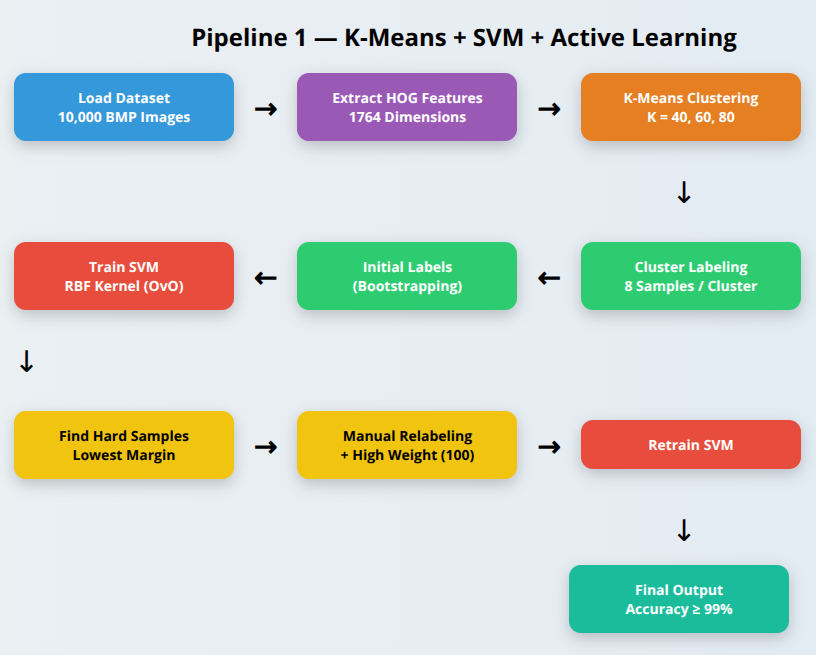
\includegraphics[width=0.95\textwidth]{Pipeline1_Flowchart.png}
\caption{Pipeline 1: K-Means + SVM + Active Learning}
\end{figure}

The pipeline consists of the following steps:
\begin{itemize}
    \item Load dataset (10,000 BMP images)
    \item Extract HOG features
    \item Apply K-Means clustering
    \item Label clusters (bootstrapping)
    \item Train SVM classifier
    \item Apply active learning for refinement
\end{itemize}

% =========================
% FEATURE EXTRACTION
% =========================
\section{Feature Extraction}

Histogram of Oriented Gradients (HOG) was used to extract features from images.

\begin{itemize}
    \item Image size: 32 × 32
    \item Feature vector size: 1764
\end{itemize}

\begin{figure}[H]
\centering
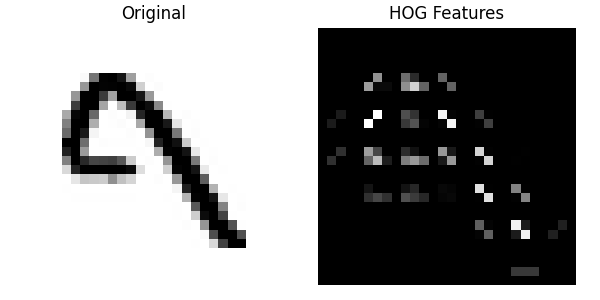
\includegraphics[width=0.7\textwidth]{HOG_Feature.png}
\caption{Example of HOG Feature Representation}
\end{figure}

% =========================
% CLUSTERING
% =========================
\section{K-Means Clustering}

K-Means clustering was applied with different values of K:

\begin{itemize}
    \item K = 40
    \item K = 60
    \item K = 80
\end{itemize}

\begin{figure}[H]
\centering
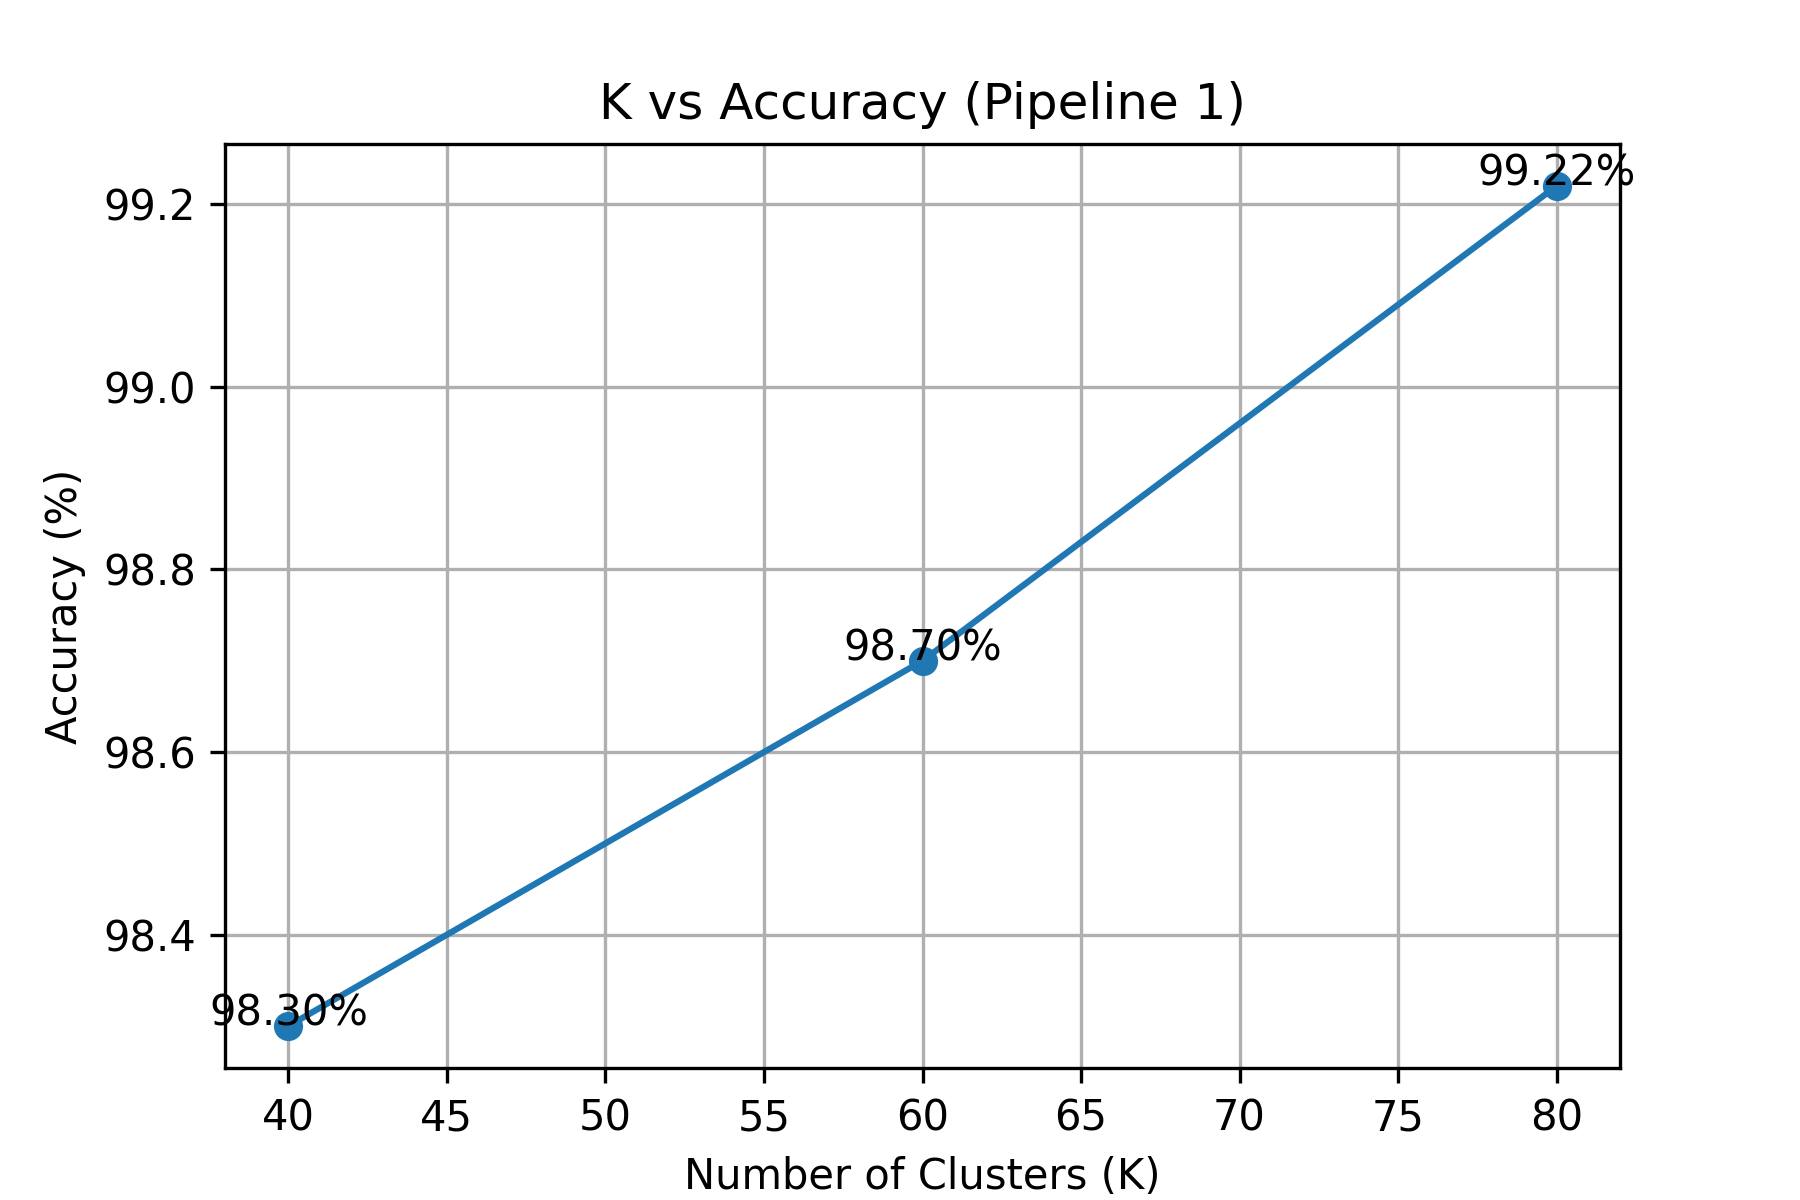
\includegraphics[width=0.7\textwidth]{k_vs_accuracy.png}
\caption{K vs Accuracy Before SVM}
\end{figure}

% =========================
% SVM AND ACTIVE LEARNING
% =========================
\section{SVM and Active Learning}

A multi-class SVM with RBF kernel (One-vs-One strategy) was used.

Active learning was applied as follows:
\begin{itemize}
    \item Select 30 least confident samples (lowest margin)
    \item Relabel manually
    \item Assign weight = 100
    \item Retrain SVM
\end{itemize}

The process stops when:
\begin{itemize}
    \item Accuracy $\geq 99\%$
    \item Improvement $< 0.1\%$
\end{itemize}

\begin{figure}[H]
\centering
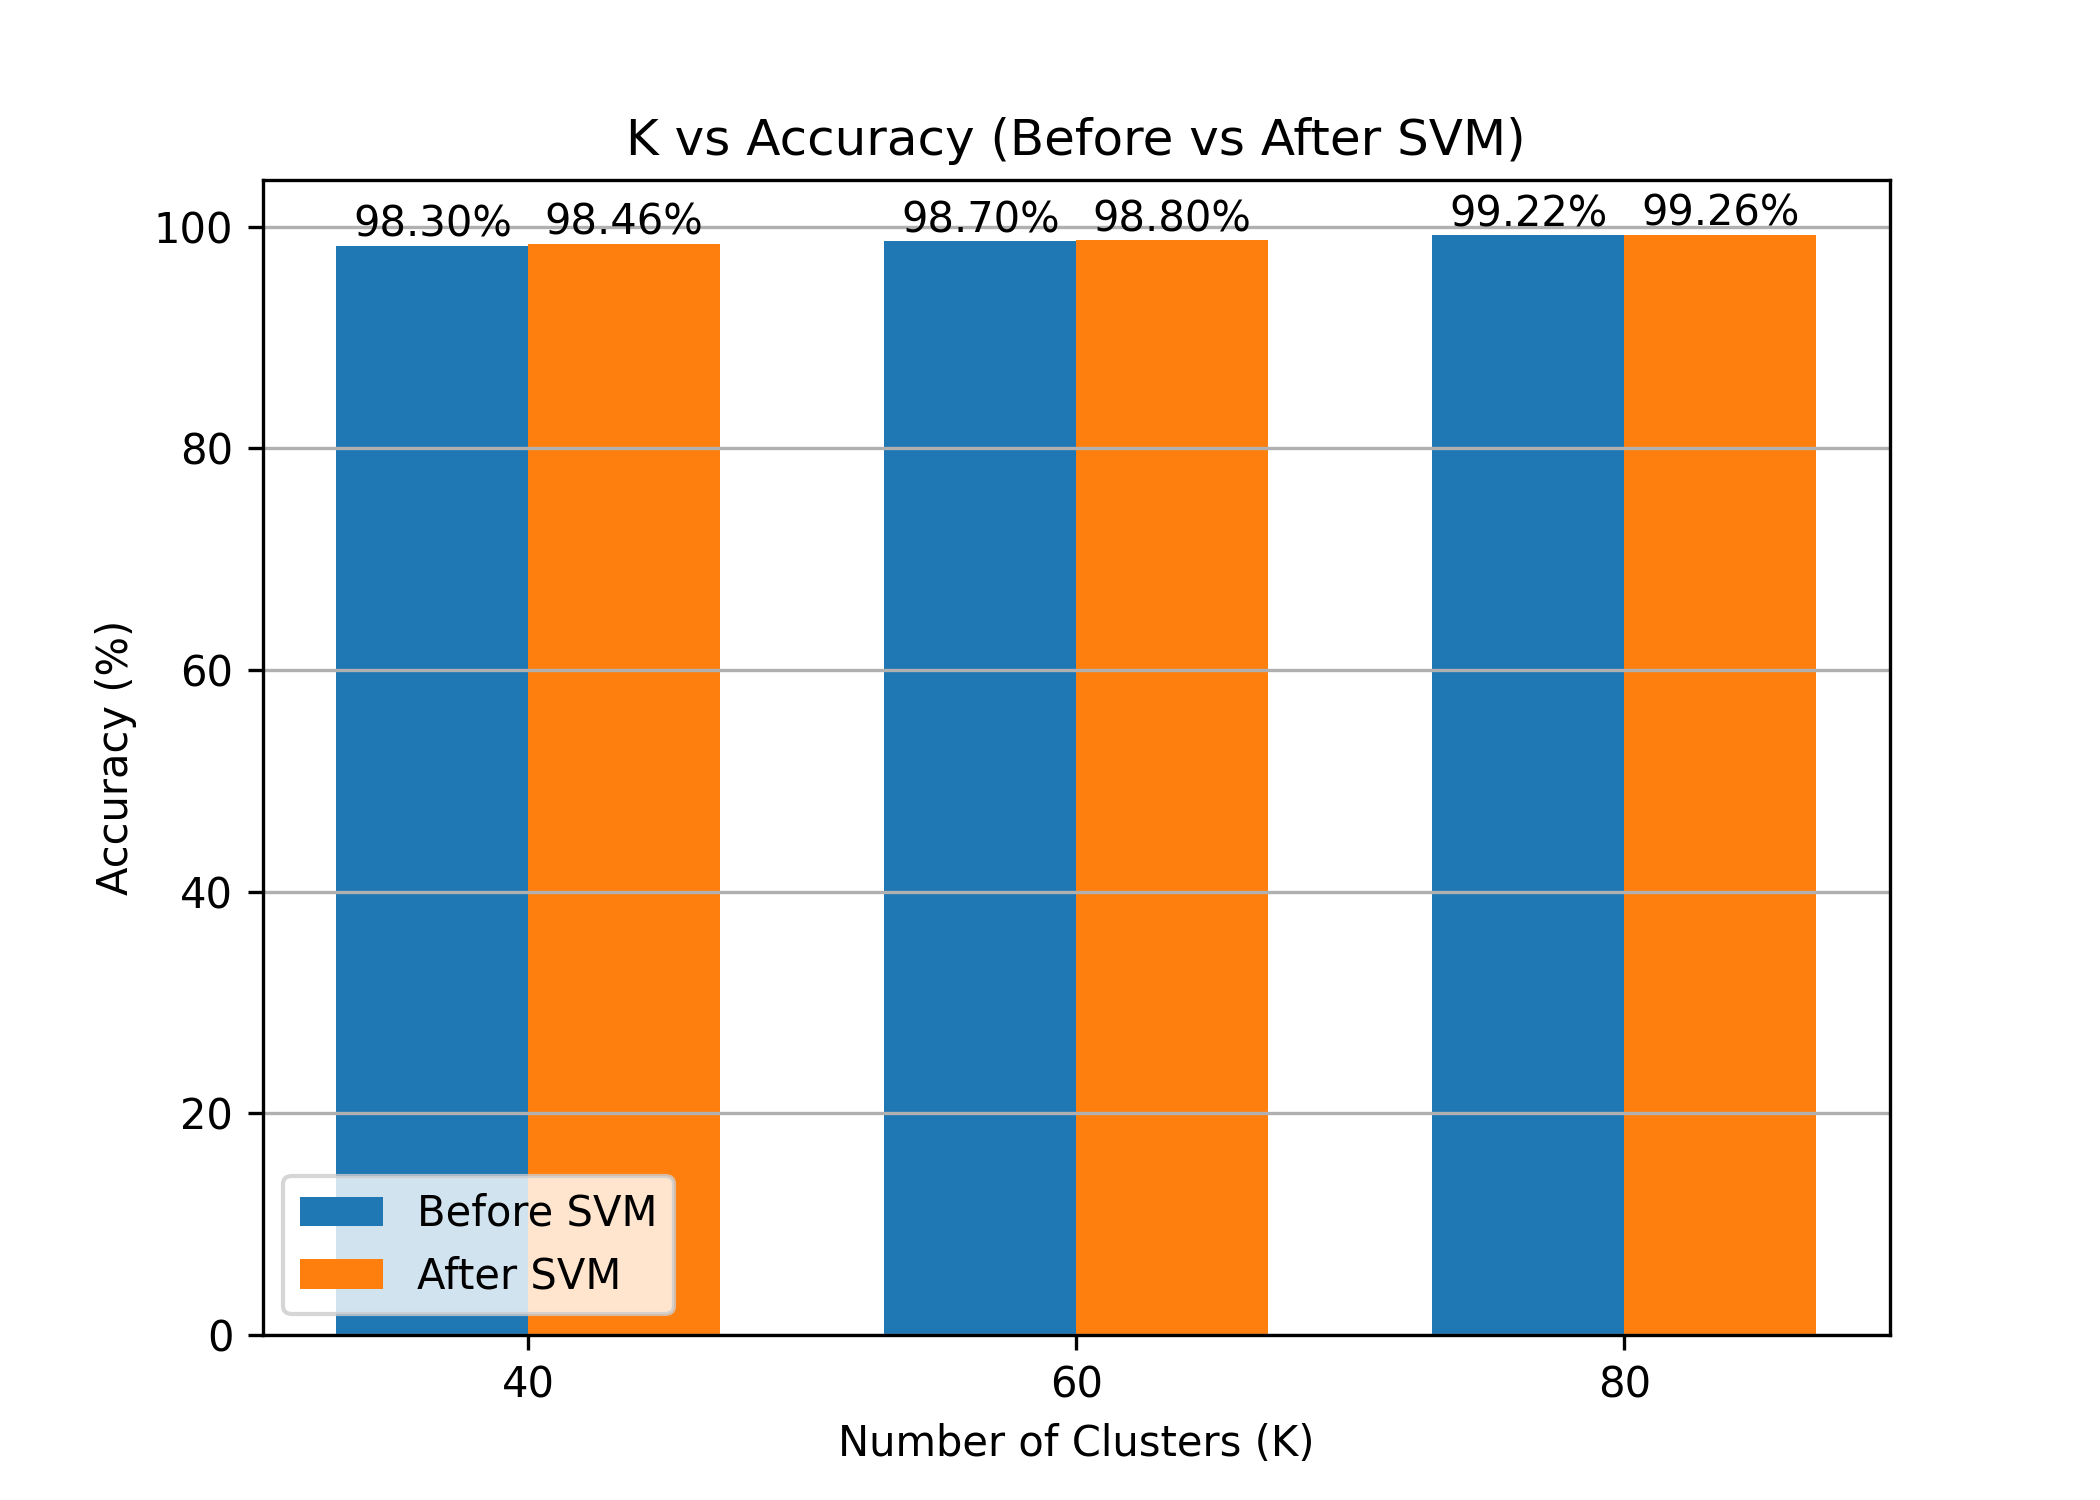
\includegraphics[width=0.7\textwidth]{svm_bar_chart.png}
\caption{Accuracy Before vs After SVM}
\end{figure}

% =========================
% RESULTS
% =========================
\section{Results}

\subsection{Accuracy}

\begin{table}[H]
\centering
\begin{tabular}{ccc}
\toprule
K & Before SVM (\%) & After SVM (\%) \\
\midrule
40 & 98.30 & 98.46 \\
60 & 98.70 & 98.80 \\
80 & 99.22 & 99.26 \\
\bottomrule
\end{tabular}
\caption{Accuracy Comparison}
\end{table}

\subsection{Iterations}

\begin{table}[H]
\centering
\begin{tabular}{cc}
\toprule
K & Iterations \\
\midrule
40 & 2 \\
60 & 2 \\
80 & 2 \\
\bottomrule
\end{tabular}
\caption{Number of Iterations}
\end{table}

% =========================
% MANUAL EFFORT
% =========================
\section{Manual Effort}

For K = 80:

\begin{itemize}
    \item Cluster labeling: 80 × 8 = 640 images
    \item Active learning: 30 × 2 = 60 images
\end{itemize}

Total images manually handled:
\[
700 \text{ images}
\]

Total time:
\begin{itemize}
    \item Cluster labeling: 1600 seconds
    \item Active learning: 600 seconds
\end{itemize}

\[
\text{Total time} = 2200 \text{ seconds} \approx 36.7 \text{ minutes}
\]

% =========================
% CONCLUSION
% =========================
\section{Conclusion}

The proposed pipeline significantly reduces manual labeling effort from 27.8 hours to approximately 37 minutes while achieving 99.26\% accuracy.

K-Means clustering provides strong initial labels, while SVM and active learning refine ambiguous samples. The improvement from SVM is more noticeable at lower K values, while higher K values already produce highly pure clusters.

% =========================
% PIPELINE 2
% =========================
\section{Pipeline 2: Manual Seed + Augmentation + Self-Training}

This pipeline adopts a semi-supervised learning approach starting from a small, high-quality human-labelled seed set. The model progressively expands its knowledge using data augmentation, active learning, and self-training.

% =========================
% FLOWCHART (TIKZ)
% =========================
\subsection{Pipeline Diagram}

\begin{figure}[H]
\centering
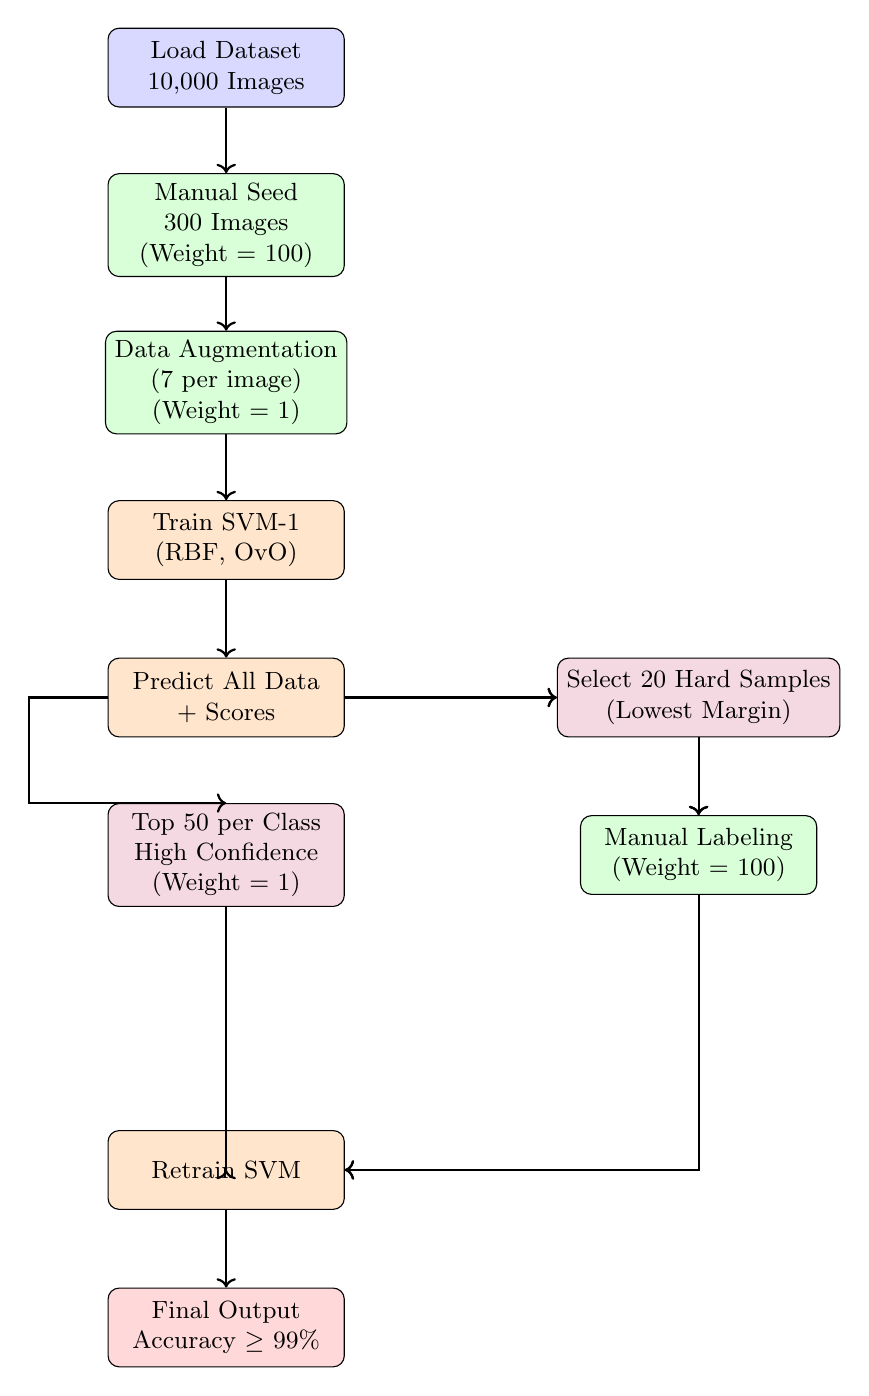
\begin{tikzpicture}[
node distance=2cm,
every node/.style={
    draw, rounded corners, align=center,
    minimum width=3cm, minimum height=1cm,
    font=\small
},
arrow/.style={->, thick},
data/.style={fill=blue!15},
process/.style={fill=green!15},
model/.style={fill=orange!20},
decision/.style={fill=purple!15},
output/.style={fill=red!15}
]

\node (data) [data] {Load Dataset\\10,000 Images};

\node (seed) [below of=data, process] {Manual Seed\\300 Images\\(Weight = 100)};
\node (aug) [below of=seed, process] {Data Augmentation\\(7 per image)\\(Weight = 1)};

\node (svm1) [below of=aug, model] {Train SVM-1\\(RBF, OvO)};
\node (predict) [below of=svm1, model] {Predict All Data\\+ Scores};

\node (hard) [right of=predict, xshift=4cm, decision] {Select 20 Hard Samples\\(Lowest Margin)};
\node (label) [below of=hard, process] {Manual Labeling\\(Weight = 100)};
\node (pseudo) [left of=label, xshift=-4cm, decision] {Top 50 per Class\\High Confidence\\(Weight = 1)};

\node (retrain) [below of=predict, yshift=-4cm, model] {Retrain SVM};

\node (output) [below of=retrain, output] {Final Output\\Accuracy $\geq$ 99\%};

\draw[arrow] (data) -> (seed);
\draw[arrow] (seed) -> (aug);
\draw[arrow] (aug) -> (svm1);
\draw[arrow] (svm1) -> (predict);

\draw[arrow] (predict) -> (hard);
\draw[arrow] (hard) -> (label);
\draw[arrow] (label) |- (retrain);

\draw[arrow] (predict.east) -- ++(1,0) |- (hard.west);
\draw[arrow] (predict.west) -- ++(-1,0) |- (pseudo.north);

\draw[arrow] (hard) -> (label);
\draw[arrow] (label) |- (retrain);

\draw[arrow] (pseudo) |- (retrain);

\draw[arrow] (retrain) -> (output);



\end{tikzpicture}
\caption{Pipeline 2: Semi-Supervised Learning Framework}
\end{figure}


% =========================
% RESULTS
% =========================
\subsection{Final Results}

\begin{table}[H]
\centering
\begin{tabular}{cc}
\toprule
Metric & Value \\
\midrule
Final Accuracy & 98.87\% \\
Iterations & 2 \\
Manual Labels & 340 \\
Pseudo Labels & 1000 \\
Estimated Time & 56.67 minutes \\
\bottomrule
\end{tabular}
\caption{Pipeline 2 Performance Summary}
\end{table}

\subsection{Iteration Progress}

Detailed iteration results are stored in the generated CSV file:

\texttt{pipeline2\_iterations.csv} :contentReference[oaicite:0]{index=0}

Each iteration records:
\begin{itemize}
    \item Accuracy improvement
    \item Number of pseudo-labelled samples
    \item Number of manually labelled samples
\end{itemize}



% =========================
% VISUALIZATION
% =========================
\subsection{Visualization}

\begin{figure}[H]
\centering
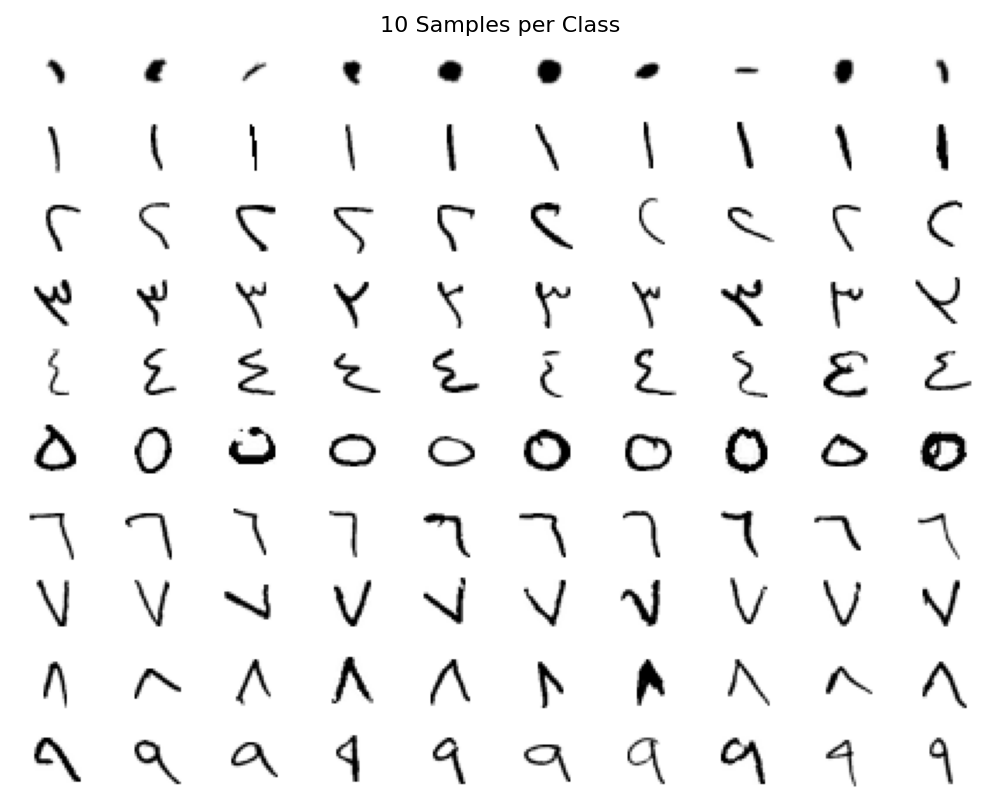
\includegraphics[width=0.8\textwidth]{Human_seed.png}
\caption{Initial Human Seed Samples (10 per class)}
\end{figure}

\begin{figure}[H]
\centering
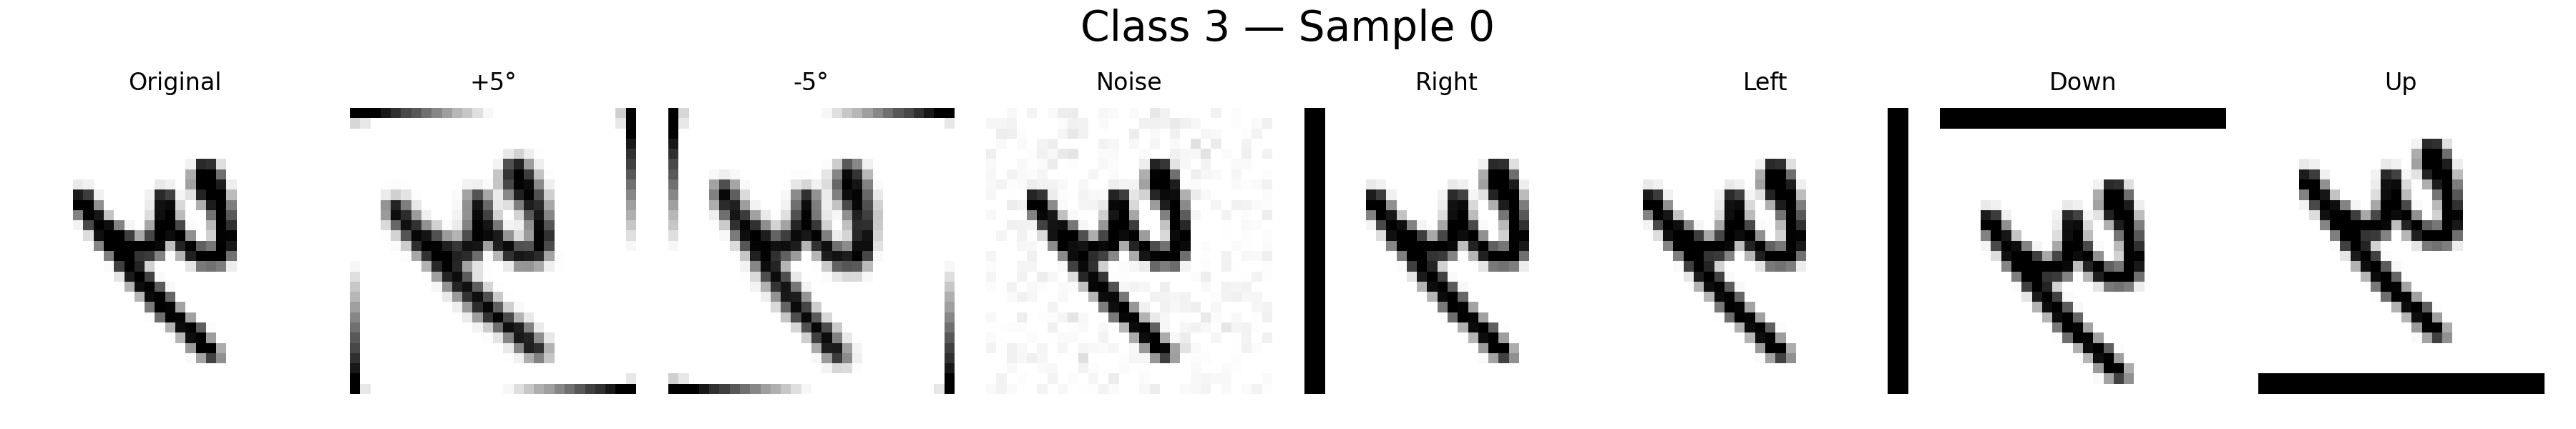
\includegraphics[width=0.8\textwidth]{class_3_sample_0.png}
\caption{Example of Data Augmentation (7 variants)}
\end{figure}

\begin{figure}[H]
\centering
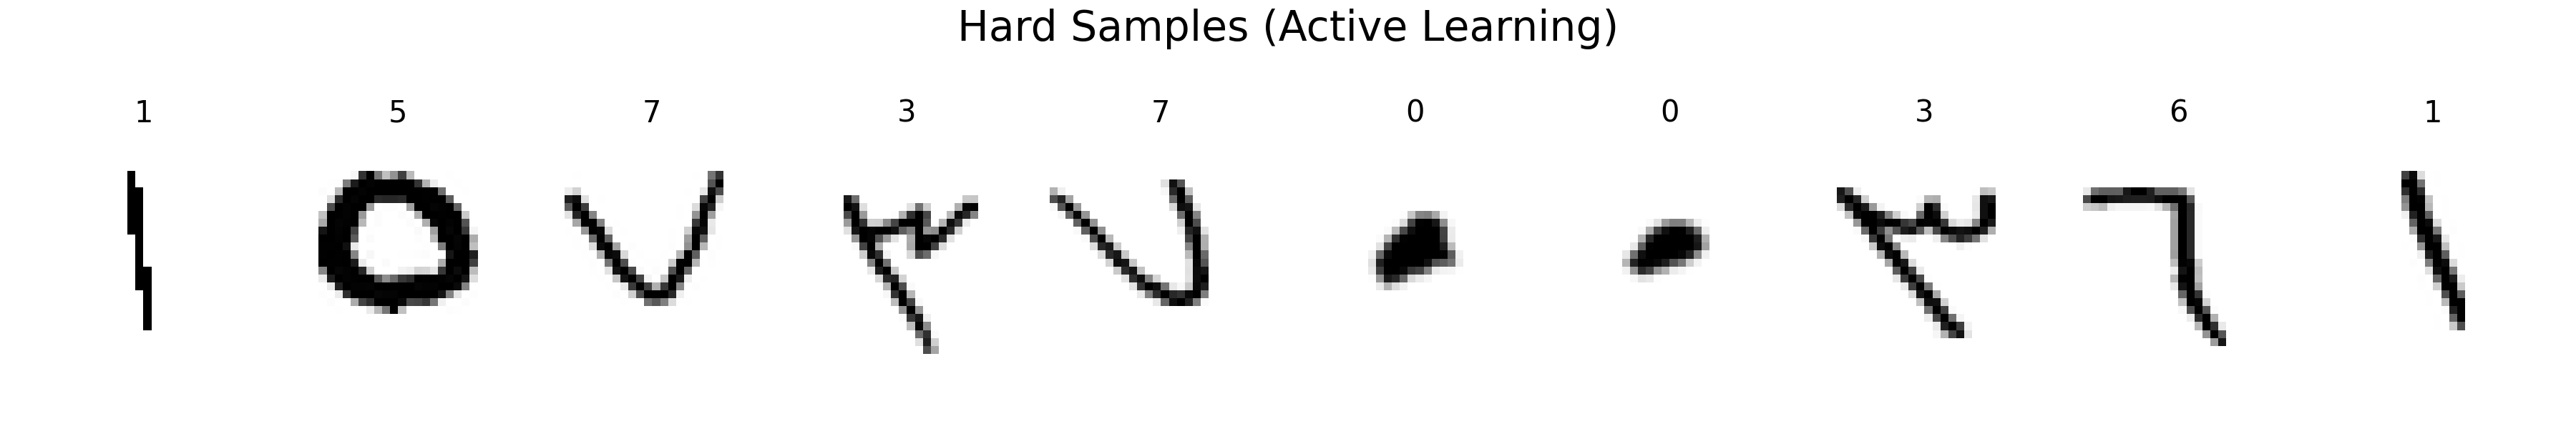
\includegraphics[width=0.9\textwidth]{hard_samples_iter_1.png}
\caption{Hard Samples (Iteration 1)}
\end{figure}

\begin{figure}[H]
\centering
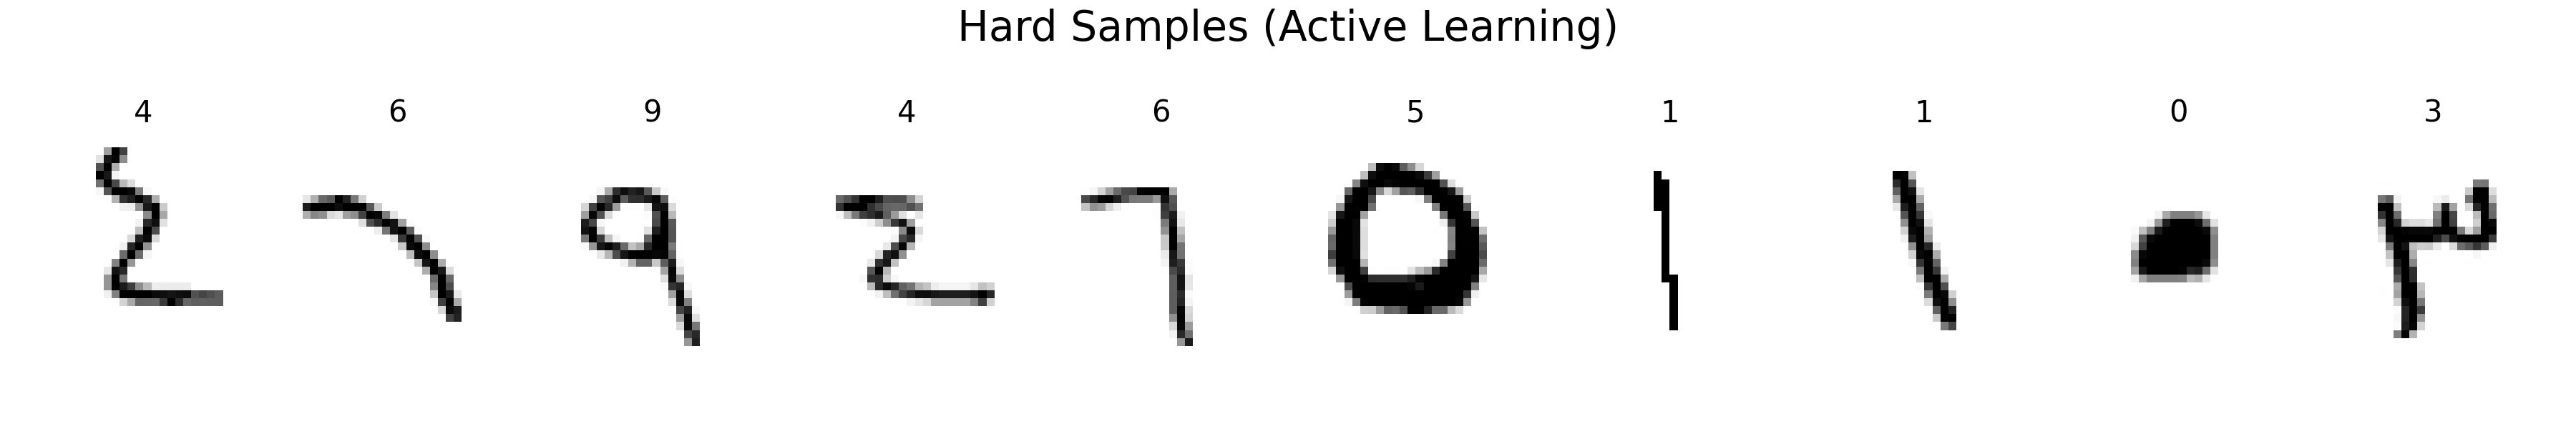
\includegraphics[width=0.9\textwidth]{hard_samples_iter_2.png}
\caption{Hard Samples (Iteration 2)}
\end{figure}

% =========================
% MANUAL EFFORT
% =========================
\subsection{Manual Effort}

Manual labeling consists of:

\begin{itemize}
    \item Initial seed: 300 images
    \item Active learning: $20 \times 2 = 40$ images
\end{itemize}

Total manual labels:
\[
300 + 40 = 340
\]

Estimated time:
\[
340 \times 10 = 3400 \text{ seconds} \approx 56.67 \text{ minutes}
\]

% =========================
% COMPARISON
% =========================
\subsection{Comparison with Pipeline 1}

\begin{table}[H]
\centering
\begin{tabular}{ccc}
\toprule
Metric & Pipeline 1 & Pipeline 2 \\
\midrule
Accuracy & 99.26\% & 98.87\% \\
Manual Images & 700 & 340 \\
Manual Time & 36.7 min & 56.7 min \\
Iterations & 2 & 2 \\
\bottomrule
\end{tabular}
\caption{Pipeline Comparison}
\end{table}

Pipeline 1 achieves higher accuracy due to clustering-based initialization, while Pipeline 2 significantly reduces manual labeling effort by leveraging self-training. However, Pipeline 2 requires slightly more total time due to per-image labeling cost.

% =========================
% CONCLUSION
% =========================
\subsection{Discussion}

Pipeline 2 demonstrates the effectiveness of semi-supervised learning. Starting from a small, high-quality seed set, the model successfully expands its training data using both active learning and self-training.

Although the final accuracy (98.87\%) is slightly below Pipeline 1, the reduction in manual labeling effort is significant. This pipeline better reflects real-world scenarios where labeled data is scarce and expensive.

The combination of:
\begin{itemize}
    \item Human supervision (high confidence)
    \item Model confidence (self-training)
    \item Iterative refinement
\end{itemize}

creates a scalable and efficient labeling strategy.

\end{document}